\chapter[DSB-SC using multiplier IC AD633]{DSB-SC using multiplier IC AD633}
\label{chapdsbsc}
\section*{Aim}
To set up a balanced modulator circuit for double side band suppressed carrier amplitude modulator.
\section*{Theory}
DSB-SC is a kind of amplitude modulation in which the carrier frequency component is absant. It is generated by multiplying the carrier and maodulating signals. If $e_c$ is the carrier and $e_m$is the message signal, where
\begin{equation}
e_c=E_c\  sin\ 2\pi f_ct
\end{equation}
\begin{equation}
e_m=E_m\  sin\ 2\pi f_mt
\end{equation}
Multiplication is done using AD633 (See \ref{AD633}) multiplier IC.
Applying $e_c$ to $\textbf{X}$ and $e_m$ to $\textbf{Y}$ with $\textbf{Z}$ is grounded, 
\begin{equation}
W= \frac{e_me_c}{10} =\frac{Emsin(2\pi f_mt).Ecsin(2\pi f_ct)}{10}
\end{equation}
\begin{equation}
W= \frac{E_mE_c}{10} \frac{[cos 2\pi (f_c\ -\ f_m)t-cos 2\pi (f_c\ +\ f_m)t]}{2}
\end{equation}
\begin{equation}
W= \frac{E_mE_c [cos 2\pi (f_c\ -\ f_m)t]}{20}- \frac{E_mE_c[cos 2\pi (f_c\ +\ f_m)t]}{20}
\end{equation}
This wave contains both the sidebands at $f_c-f_m$ and $f_c+f_m$, but not the wave at carrier frequency\footnote{$sin \ A.\ sin\ B=\frac{cos\ (A-B)-cos\ (A+B)}{2}$}. Hence the name double sideband suppressed carrier modulation(DSB-SC).
\section*{Design}

To the \textbf{X} input of the IC, feed the carrier sinusoid of amplitude $E_m=2.5\ V$ and frequency $f_m= 1\ kHz$.\\

To the \textbf{Y} input of the IC, feed the message sinusoid of amplitude $E_c=2.5\ V$ and frequency $f_c= 10\ kHz$.\\
Ground the \textbf{Z} input of the IC.\\
Provide the biasing voltage of +15 V to pin 8 of the IC and -15 V to pin 5 of the IC.\\

The output AM signal will have a waveform as given by,

\begin{equation}
W=\frac{X.Y}{10}+Z
\end{equation}
\begin{equation}
W=\frac{e_m.e_c}{10}=\frac{(2.5) \ .(2.5)}{10}\frac{[cos 2\pi9000t-cos 2\pi11000t]}{2}
\end{equation}

\begin{equation}
W=\frac{6.25}{20}[cos 2\pi9000t-cos 2\pi11000t]
\end{equation} 

\section*{Circuit Diagram}
The circuit diagram for implementing DSBSC using multiplier IC is shown in figure \ref{DSBSCckt}.
\begin{figure}[h]
\begin{center}
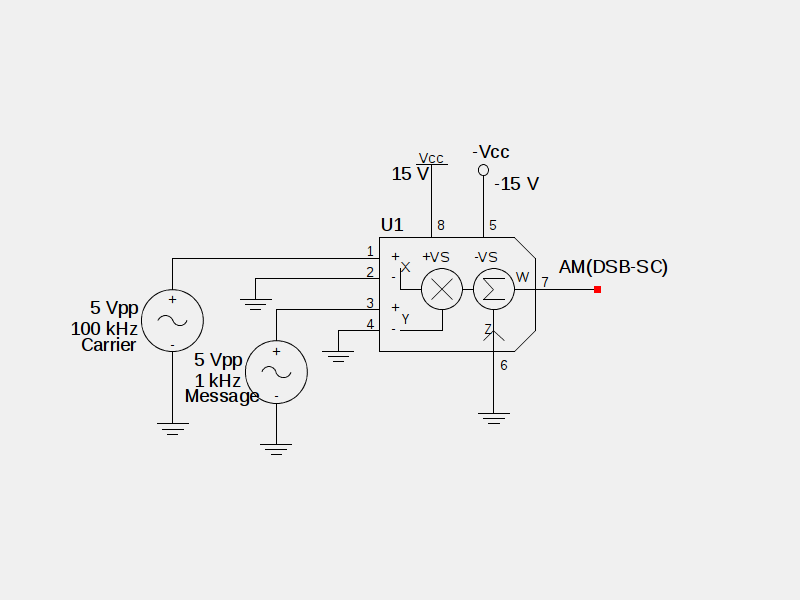
\includegraphics[width=14cm,height=8cm,trim=2cm 4cm 2cm 4cm, clip=true]{633dsbscckt.png}
\caption{Circuit diagram for DSBSC using multiplier IC}
\label{DSBSCckt}
\end{center}

\end{figure}

\section*{Procedure}
\begin{itemize}
\item
Make connections as shown in the circuit diagram, figure \ref{DSBSCckt}.
\item
Feed the message and carrier signals.
\item
Connect the pin number 7 of the IC to a CRO and observe the resultant waveform which is DSB-SC.
\item

Plot the signals observed on a graph sheet.
\end{itemize}
\section*{Observation}

The following figure \ref{DSBSC} shows\footnote{By Serych at cs.wikipedia [Public domain], from Wikimedia Commons.  \ \url{http://commons.wikimedia.org/wiki/File\%3AAM-DSBSC.png}} the DSB-SC signal in blue and the original message is shown in red. (\emph{It is an indicative graph, not to scale as per the experimental set-up.})
\begin{figure}[h]
\begin{center}
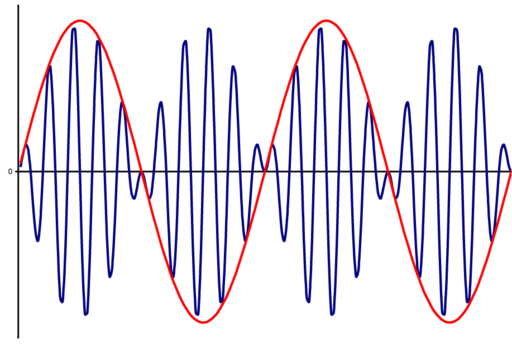
\includegraphics[width=10cm,height=4cm]{AMDSBSC.png}
\caption{DSB-SC signal in blue, original message shown in red.}
\label{DSBSC}
\end{center}

\end{figure}


\section*{Result}
Implemented DSB-SC using multiplier IC AD 633 and observed the signal waveforms.